\section{Local Linear Embedding} 

  PCA and MDS are linear embedding methods. Let's move onto nonlinear ones. The first nonlinear models that we work with again use the idea of locality (remember kernel regression). You have data that is globally nonlinear, but if you look at a point and its local neighborhood around it, then it is approximately linear since we assume that it lives in some smooth manifold. 

  \begin{figure}[H]
    \centering 
    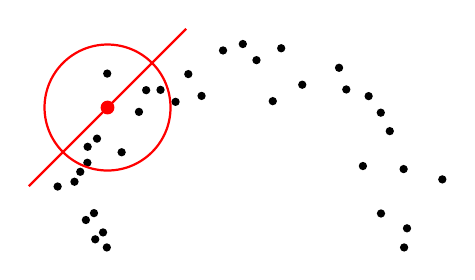
\begin{tikzpicture} 
      \pgfmathsetseed{42}
      % Draw half spiral (from 0 to 180 degrees) with more points
      \foreach \t in {0,5,...,180} {
        \pgfmathsetmacro{\radius}{2.5 - \t/120}
        \pgfmathsetmacro{\noise}{1.0*rnd}
        \pgfmathsetmacro{\x}{(\radius + \noise) * cos(\t)}
        \pgfmathsetmacro{\y}{(\radius + \noise) * sin(\t)}
        
        \fill (\x, \y) circle (1.5pt);
        
        % Store coordinates of 25th point (t=120, since we start at 0 and increment by 5)
        \ifnum\t=120
          \fill[red] (\x, \y) circle (2.5pt);
          \pgfmathsetmacro{\centerx}{\x}
          \pgfmathsetmacro{\centery}{\y}
          \global\let\circlecenterx\centerx
          \global\let\circlecentery\centery
        \fi
      }
      
      % Add red circle centered on the 25th point
      \draw[red, thick] (\circlecenterx, \circlecentery) circle (0.8);
      
      % Add red line cutting through the circle area
      \draw[red, thick] (\circlecenterx - 1, \circlecentery - 1) -- (\circlecenterx + 1, \circlecentery + 1);
    \end{tikzpicture}
    \caption{Local linear embedding assumes that the data is locally linear. } 
    \label{fig:local_linear_embedding}
  \end{figure}

  The concept of neighborhood can be defined in two ways. You can either just fix an $\epsilon$ and take the $\epsilon$-ball around each point $x_i$. Or you can fix a $k$ and take the $k$ nearest neighbors of each point. The general idea of using kernel PCA is to take a local neighborhood of the data and construct some linear approximation of it. 

